\chapter{Experimental Results}
\label{cha:experimental_results}

\section{2D Density Esitmation}

For the GMM I used three functions that generate two dimensional data in some specific pattern with some added random noise. These 
can be seen as the true data generating distribution and the goal is to model this distribution using the GMM with the discussed 
algorithms. 

Using these I generated 20,000 datapoints and split them evenly into a train and a test dataset. Note that usually the test dataset is smaller 
than the training dataset due to limited data availability but since we can basically generate unlimited samples if we know 
the data generating distribution, I decided to split them in this way. 
The training samples can be seen in Figure \ref{fig:2d_datasets}. \\

\begin{figure}[h]
    \centering
    \makebox[\textwidth][c]{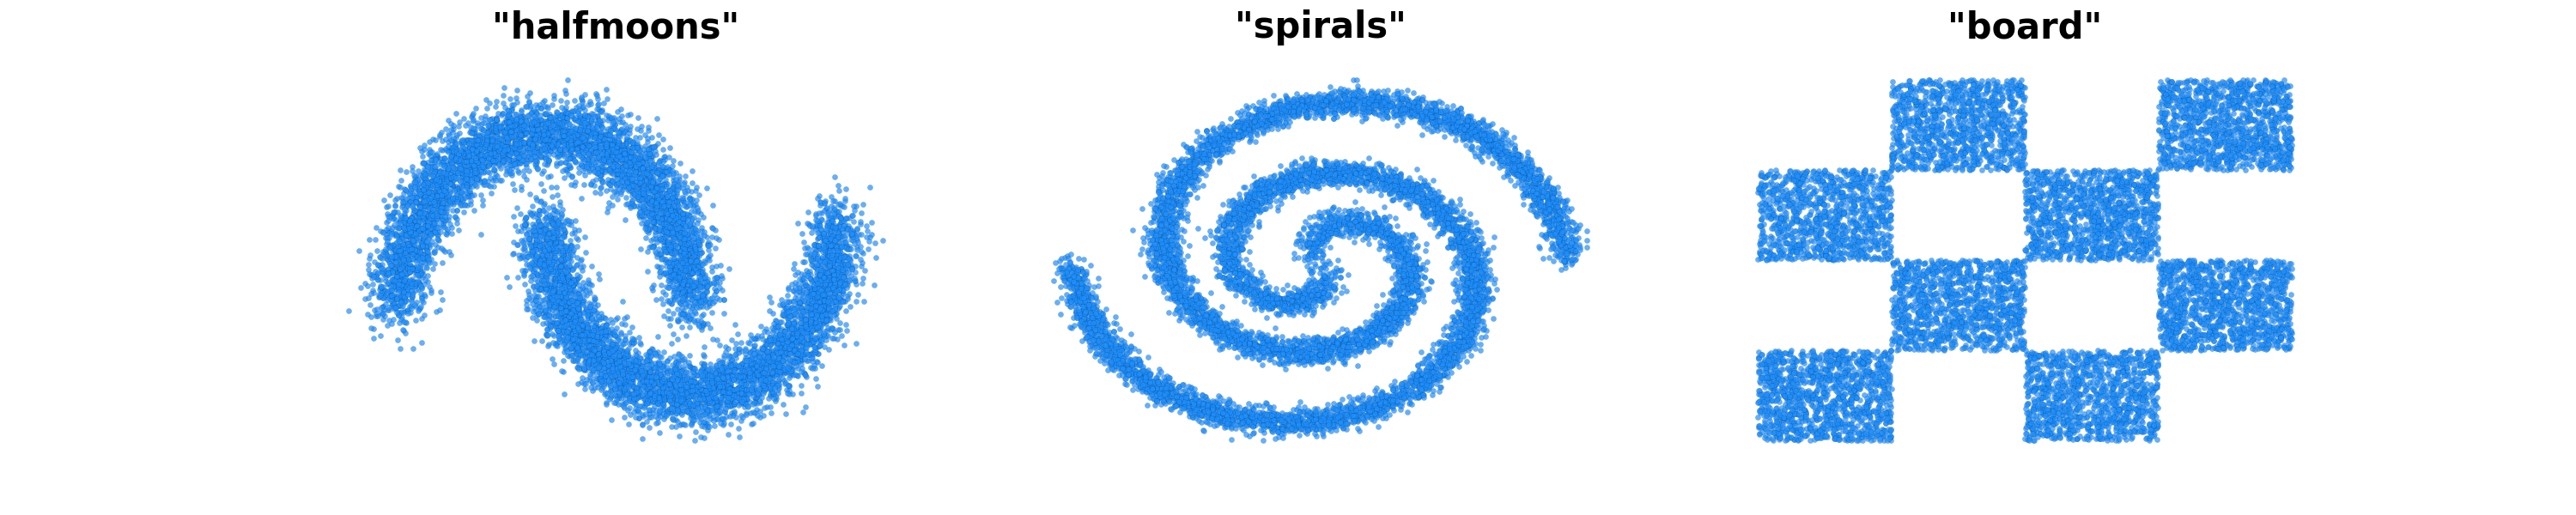
\includegraphics[width=1.2\textwidth]{figures/datasets.png}}
    \caption{2D Samples for all three distributions}
    \label{fig:2d_datasets}
\end{figure}

\begin{figure}[H]
    \centering
    \makebox[\textwidth][c]{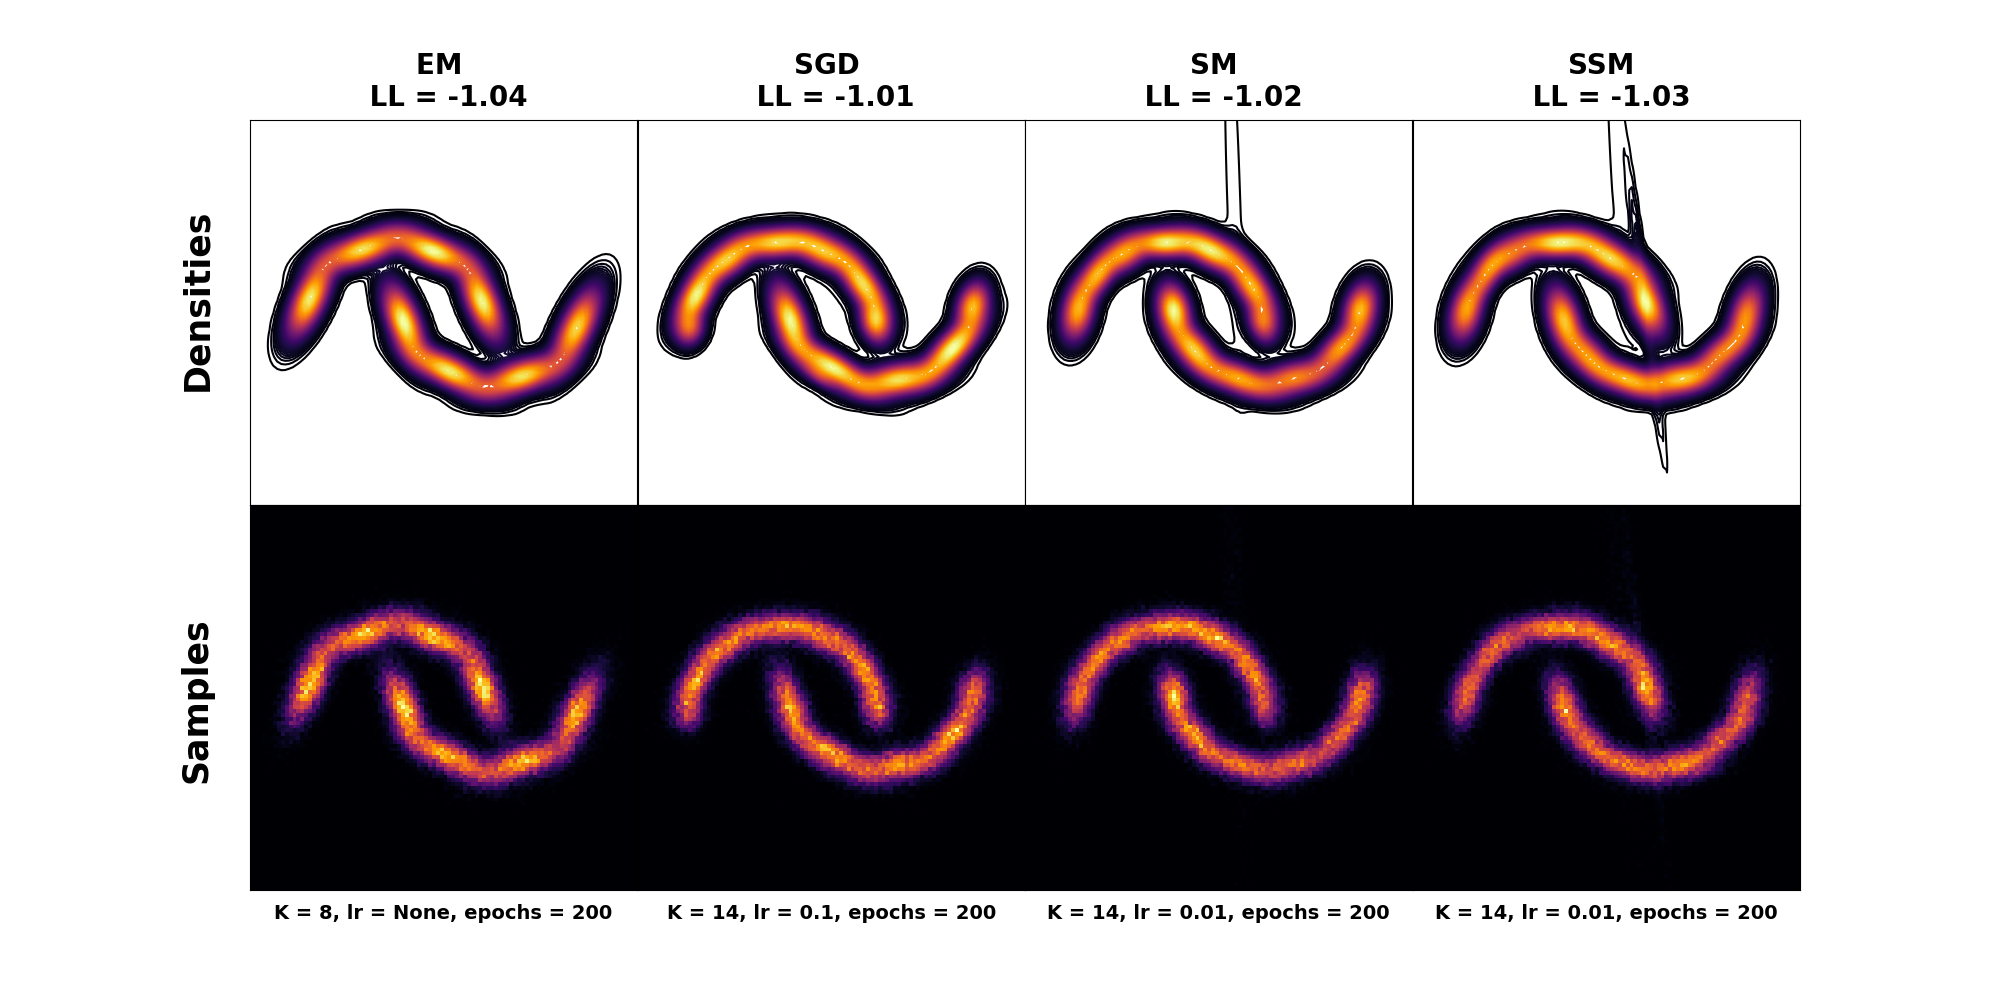
\includegraphics[width=1.2\textwidth]{figures/moons_best_ds.png}}
    \caption{Densities and Samples for "Halfmoons" with best hyperparameters for each algorithm}
    \label{fig:moons_best}
\end{figure}

\begin{figure}[H]
    \centering
    \makebox[\textwidth][c]{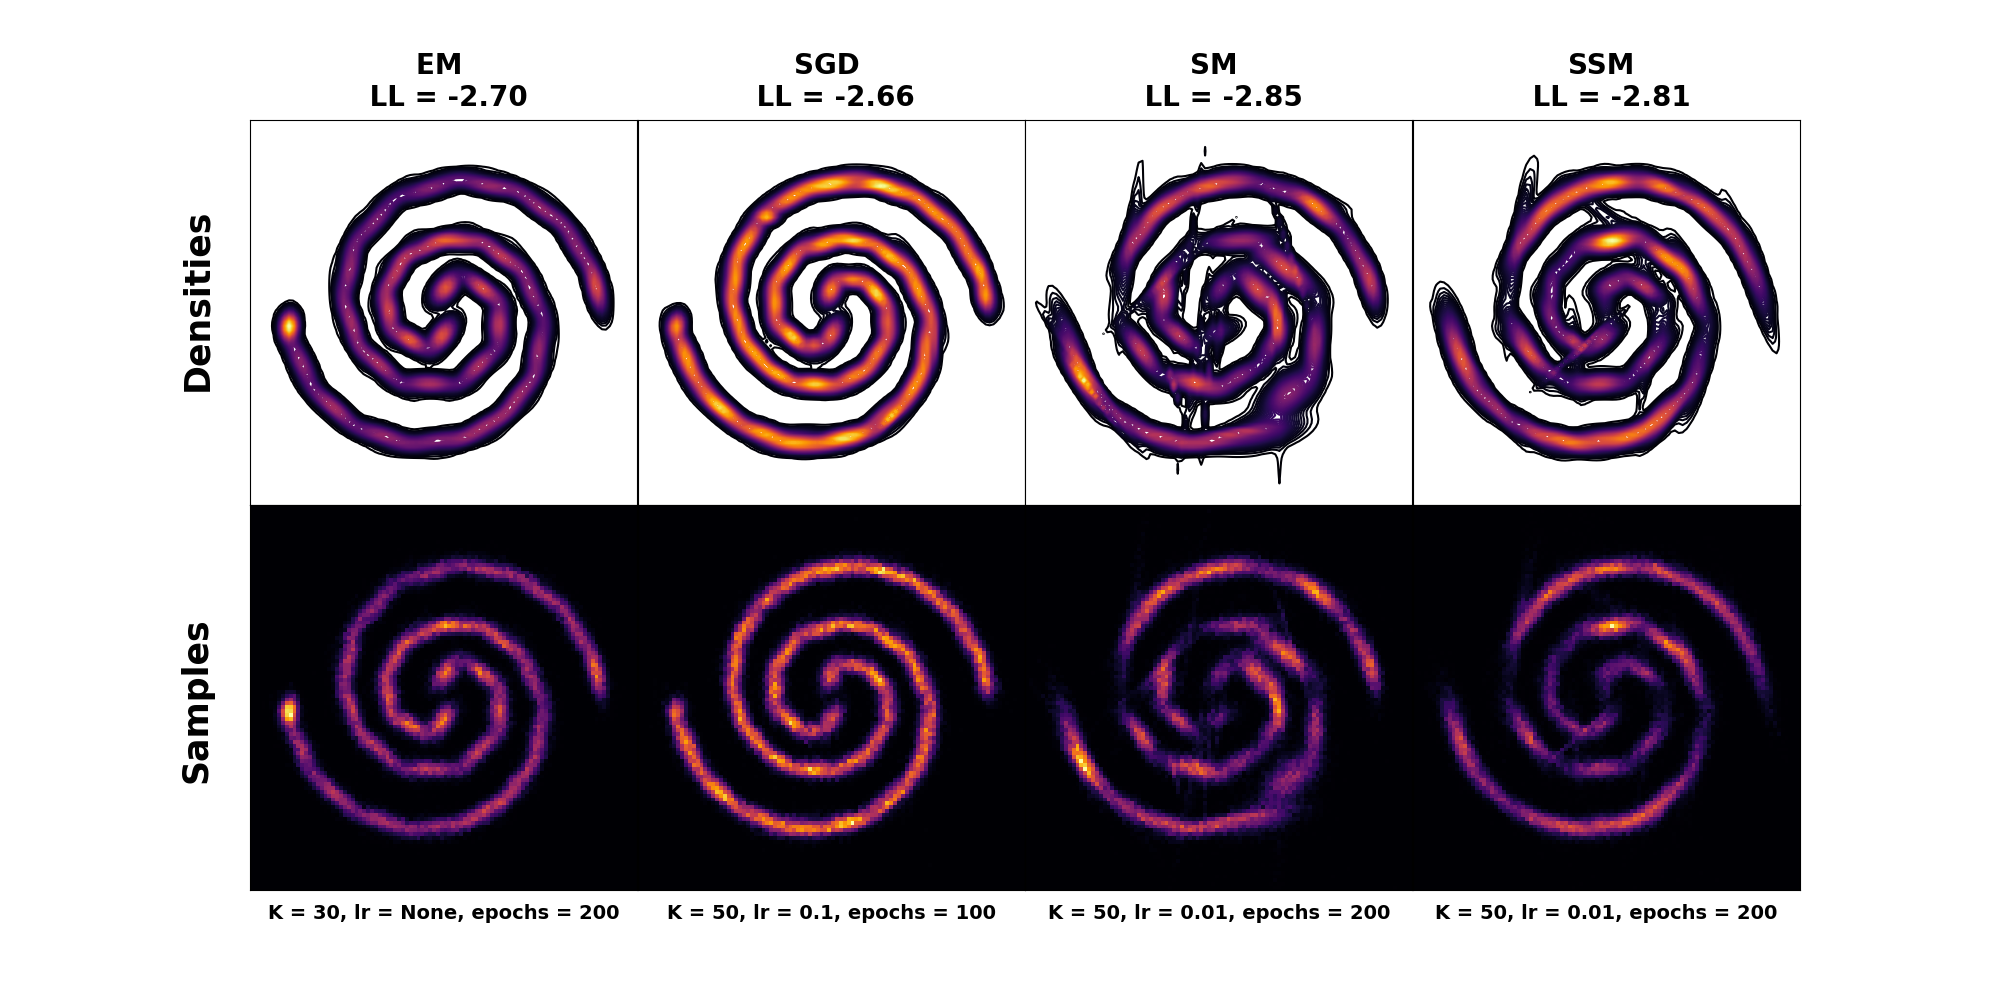
\includegraphics[width=1.2\textwidth]{figures/spirals_best_ds.png}}
    \label{fig:spirals_best}
    \caption{Densities and samples for "Spirals" with best hyperparameters for each algorithm}
\end{figure}

\begin{figure}[H]
    \centering
    \makebox[\textwidth][c]{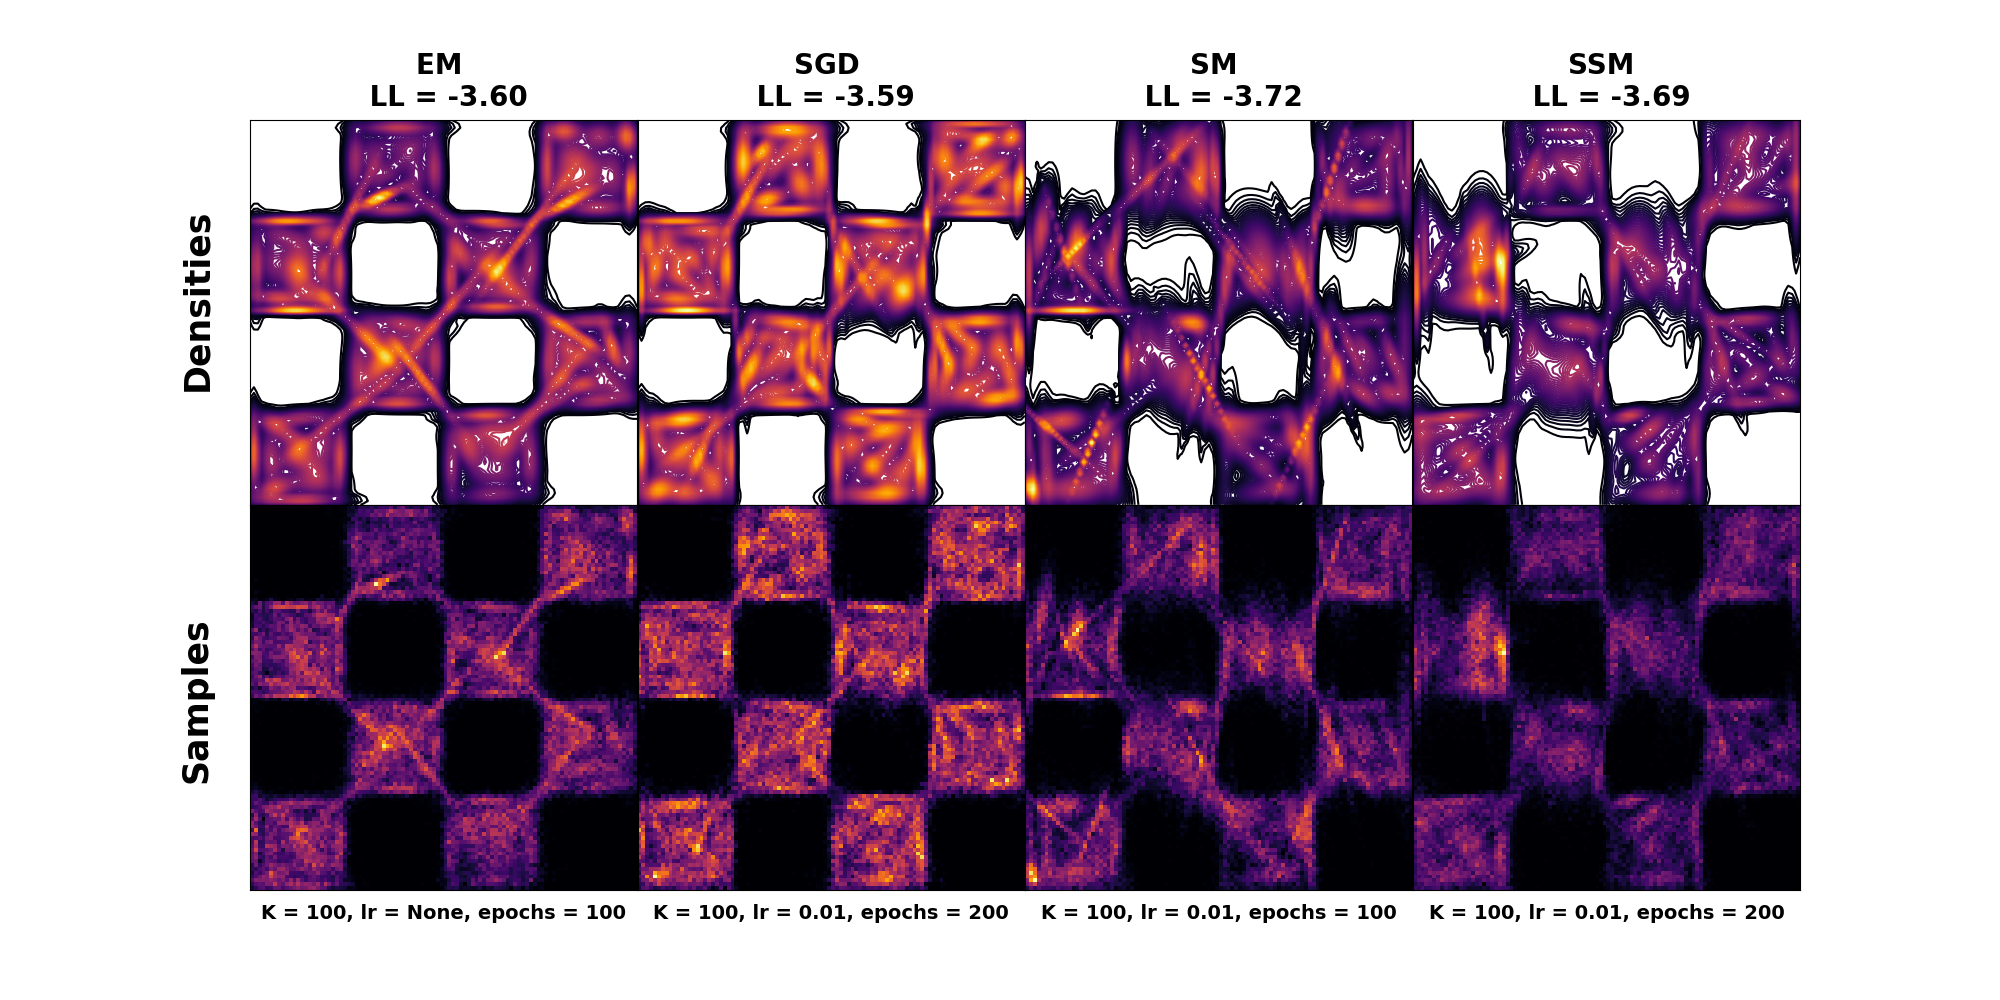
\includegraphics[width=1.2\textwidth]{figures/board_best_ds.png}}
    \label{fig:board_best}
    \caption{Densities and samples for "Board" with best hyperparameters for each algorithm}
\end{figure}


% \newpage
\section{Images Density Estimation}

I used the MNIST Dataset \cite{mnist} 

\begin{figure}[htb]
    \centering
    % First subfigure
    \begin{subfigure}[b]{0.3\textwidth}
        \centering
        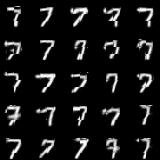
\includegraphics[width=\textwidth]{figures/mnist_EM.png} % replace with your image file
        \caption{EM}
        \label{fig:sub1}
    \end{subfigure}
    \hfill
    % Second subfigure
    \begin{subfigure}[b]{0.3\textwidth}
        \centering
        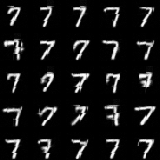
\includegraphics[width=\textwidth]{figures/mnist_SGD.png} % replace with your image file
        \caption{SGD}
        \label{fig:sub2}
    \end{subfigure}
    \hfill
    % Third subfigure
    \begin{subfigure}[b]{0.3\textwidth}
        \centering
        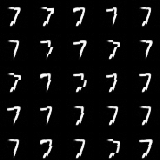
\includegraphics[width=\textwidth]{figures/mnist_SSM.png} % replace with your image file
        \caption{SSM}
        \label{fig:sub3}
    \end{subfigure}

    \caption{MNIST Samples}
    \label{fig:three_images}
\end{figure}